%%%%%%%%%%%%%%%%%%%%%%%%%%%%%%%%%%%%%%%%%%%%%%%%%%%%%%%%%%%%%%%%%%%%%%%%%%%%%%%%%%%%%%%%%%%%%%%%%%%%

\chapter{Future work}
\chaptermark{future work}
\label{chapter: future work}

%%%%%%%%%%%%%%%%%%%%%%%%%%%%%%%%%%%%%%%%%%%%%%%%%%%%%%%%%%%%%%%%%%%%%%%%%%%%%%%%%%%%%%%%%%%%%%%%%%%%

In Chapters~\ref{chapter: outflow} to \ref{chapter: dendro}, this thesis presents a detailed analysis of a specific starburst: the nuclear starburst in \ngc253. It is not exhaustive and many more details of the star formation and feedback processes can be learned from the existing data and future observations. Being focused on a single galaxy, the work shown is not representative of the variety of all starbursting systems found throughout the universe.
Several aspects are therefore needed to be tackled in the future:
(1) Starbursts occur in a variety of environments that must be characterized in detail.
(2) The specific launching processes of molecular outflows are still not understood and high resolution observations across ISM phases and stellar properties are needed.
(3) Upcoming instruments will offer higher resolution data for more targets in significantly shorter time than today. To harvest this potential, improved data analysis techniques are required to cut down on time-consuming manual interaction.


%%%%%%%%%%%%%%%%%%%%%%%%%%%%%%%%%%%%%%%%%%%%%%%%%%%%%%%%%%%%%%%%%%%%%%%%%%%%%%%%%%%%%%%%%%%%%%%%%%%%

\section{The variety of starburst environments}
\label{discussion: section: starburst environments}

Massive star formation at high redshift covers a range of properties, presumably as a function of environment, as do their local analogs. In order to deepen our understanding of the star formation and related feedback processes, we need to expand the current pilot studies such as this thesis. 

One important step is to expand the sample of currently a single galaxy (\ngc253) to all sources in the local universe where similar measurements can be achieved. Limiting factors are the required parsec scale resolution and simultaneously high sensitivity to detect the fainter diagnostic spectral lines.
In the local universe, of order ten galaxies fulfill these requirements and cover a wide range of star formation/AGN properties: from pure starbursts to purely AGN dominated and combined AGN-starburst systems with non-negligible contribution of both mechanisms.
Aside from \ngc253 presented here, M82, \ngc4945 and the Circinus galaxy are the most promising targets to probe different environments.

M82 is a stronger \citep[$SFR \sim 13-33$\,\Msunyr; e.g.][]{2003ApJ...599..193F} and more evolved \citep[e.g.][]{2006ApJS..164..450M} starburst than \ngc253. M82, thus, allows to sample the more extreme range of starburst conditions. We successfully proposed for observations (P.I.: N. Krieger) in the 230\,GHz band including \co21 with NOEMA (Northern Extended Millimeter Array) in summer semester 2019 and winter semester 2019/2020 and the interferometer observations are finished as of February 2020. Accompanying single dish observations with the IRAM 30\,m telescope are scheduled for May 2020 and will contribute the sensitivity to large scale emission. With almost 100\,h of observation time, this project provides the largest, deepest and highest resolution CO mosaic of molecular gas in M82 ever obtained.

\ngc4945 at a distance of 3.6\,Mpc is very similar in its properties to \ngc253 in that it is a barred spiral of $\sim 10^{11}$\,\Msun \citep[\ngc253: $\sim 5\times10^{10}$\,\Msun][]{1991AJ....101..456P} with a central starburst. Additionally, \ngc4945 contains an AGN classified as a Seyfert~2 type. ALMA observations at $\sim 2.2$\,pc resolution are already executed (P.I.: A. Leroy) and show 27 massive stellar clusters not previously detected (Figure~\ref{discussion: figure: ngc4945 SSCs}; Emig et al., 2020, in prep.).

\begin{figure}
    \centering
    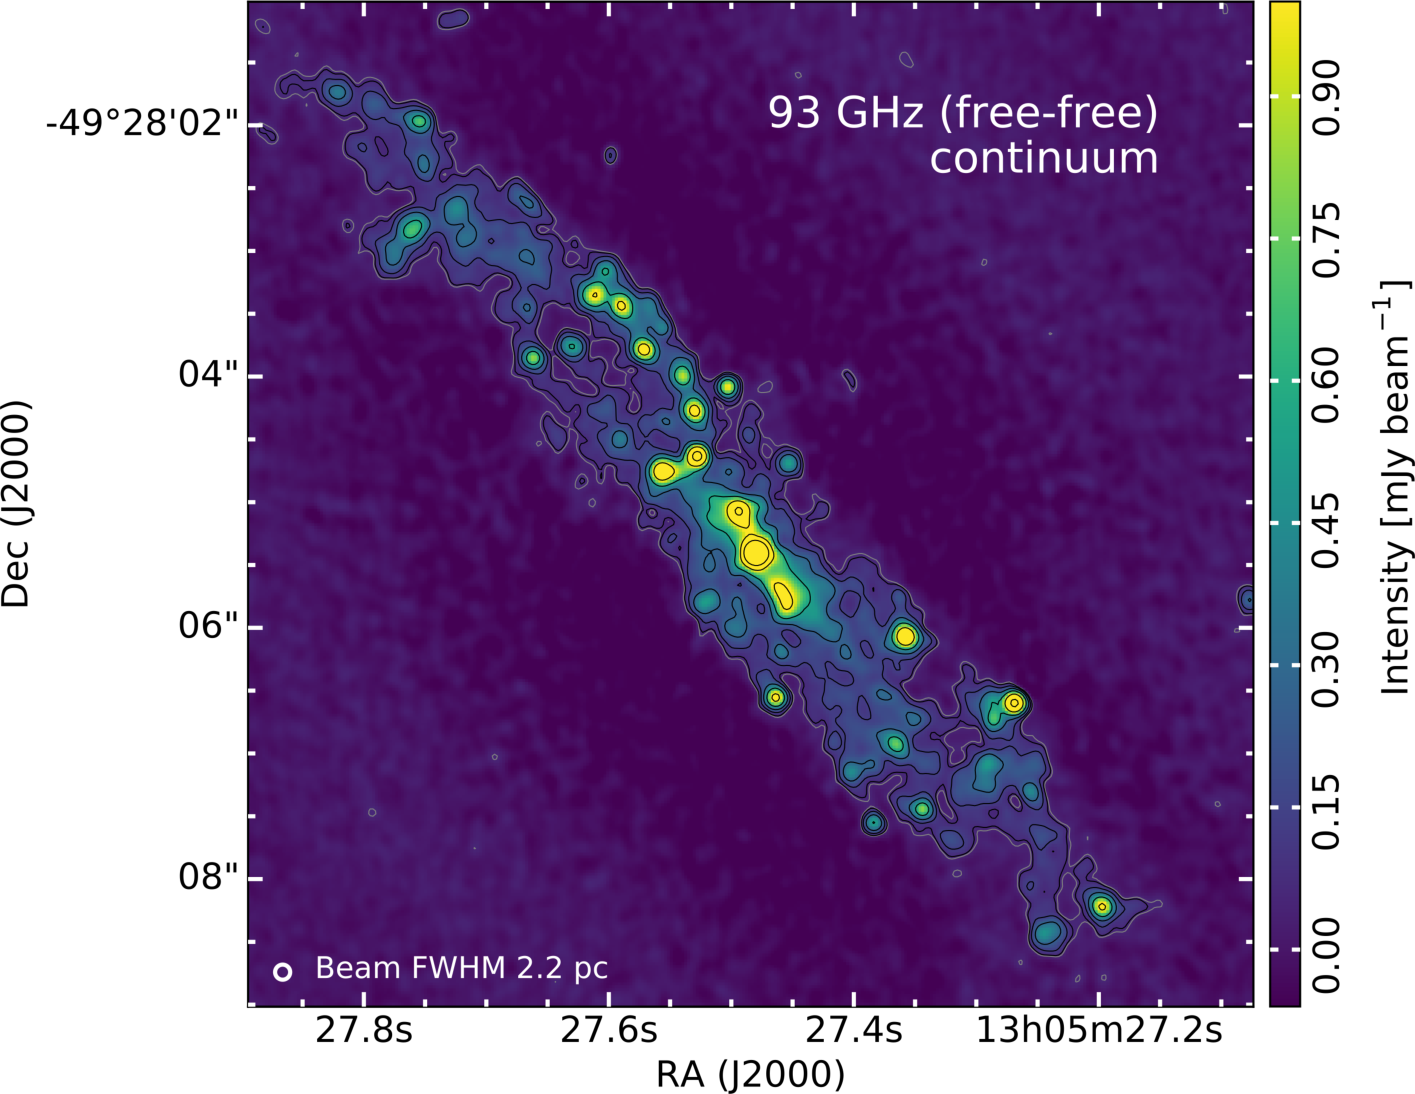
\includegraphics[width=0.6\textwidth]{thesis/images/chapters/discussion/Emig_cont93.pdf}
    \caption[Newly detected SSCs in \ngc4945]{ALMA 93\,GHz free-free continuum emission in \ngc4945 at a resolution of $\sim 2.2$\,pc. The point-sources indicate 27 newly detected SSCs (Emig et al., 2020, in prep.).
    }
    \label{discussion: figure: ngc4945 SSCs}
\end{figure}

The Circinus galaxy (ESO 97-G13) does not host a starburst and its outflow is thought to be driven primarily by the central AGN (Seyfert type~2). ALMA observation of Circinus are approved (P.I.: L. Zschaechner).

Starting with these galaxies, we will obtain a consistent sample of molecular outflows and their drivers at high spatial and spectral resolution. 


%%%%%%%%%%%%%%%%%%%%%%%%%%%%%%%%%%%%%%%%%%%%%%%%%%%%%%%%%%%%%%%%%%%%%%%%%%%%%%%%%%%%%%%%%%%%%%%%%%%%

\section{How are outflows launched and how do the outflow phases interact?}
\label{discussion: section: outflow launching}

%%%%%%%%%%%%%%%%%%%%%%%%%%%%%%%%%%%%%%%%%%%%%%%%%%%%%%%%%%%%%%%%%%%%%%%%%%%%%%%%%%%%%%%%%%%%%%%%%%%%

\subsection{Resolving outflow launching}

Before ALMA, it was merely possible to study the ISM in nearby galaxies on the size scale of GMCs. The parsec-scale resolution that we can achieve now with ALMA allows the study of ISM properties down to stellar cluster scales as we have shown in Chapters~\ref{chapter: outflow}-\ref{chapter: dendro}.
However, this is still not enough to resolve the actual launching of an outflow or wind which is expected to occur as the combined effect of stellar winds and SNe within clusters.
Chapter~\ref{chapter: outflow catalog} shows that we can now trace back individual molecular outflows to the disk and even estimate their launching site. On the other hand, it also shows that close to the disk a kinematic separation of the outflow becomes impossible using CO emission because outflow and disk begin to blend into each other.
Therefore other approaches at even higher resolution and with different tracers are needed to target individual outflow launching sites.

In order to recover the physics of outflow launching, a panchromatic study covering a wide variety of tracers is required.
The primary puzzle in outflow launching is to work out how dense molecular gas is launched.
The energetic feedback processes (stellar winds, SNe) can easily accelerate ionized gas but it remains unclear how the feedback energy and momentum is transferred to the molecular gas without destroying it. The involved energies are easily enough to dissociate or disperse the molecular gas without creating a molecular outflow.
Several potential mechanisms have been proposed in the literature that now need to be examined observationally across wavelengths and at very high resolution.

Due to the high extinction in the embedded clusters in starbursts, optical observations cannot probe potential launching mechanisms and instead infrared to radio wavelengths are required.

In the coming years, JWST will be the premier instrument to study the (super) star cluster in the centers of nearby starbursts in NIR and MIR. 
We are currently preparing JWST observations to enter GO cycle~1 with the May 2020 deadline for proposals. 
Figure~\ref{discussion: figure: JWST planing} shows the planned observational setup for \ngc253 but the observations will further target M82.  The MIRI MRS imager for mid-inrared (MIR) photometry and the NIRSpec (near-infrared) integral field unit (IFU) will provide kinematic information of the stellar content.
The achieved spatial and spectral resolution ($\sim$1\,pc) of these instruments will closely match the existing ALMA data. The NIR/MIR range probes dust and will provide crucial parameters such as the distribution traced by PAH emission in and around the stellar clusters. 
Combined with the molecular gas data, these observations will allow us to test, for instance, the model of momentum transfer through dust grains \citep[e.g.][]{2018ApJ...854..110Z}.
NIRSpec IFU observations will complement the dense gas kinematics obtained from the kinematic decomposition analysis in Chapter~\ref{chapter: outflow} with stellar kinematics and a comparison of the two will shed light on the interaction between forming stellar clusters and surrounding gas (accretion onto the clusters and the launching of molecular outflows).

\begin{figure}
    \centering
    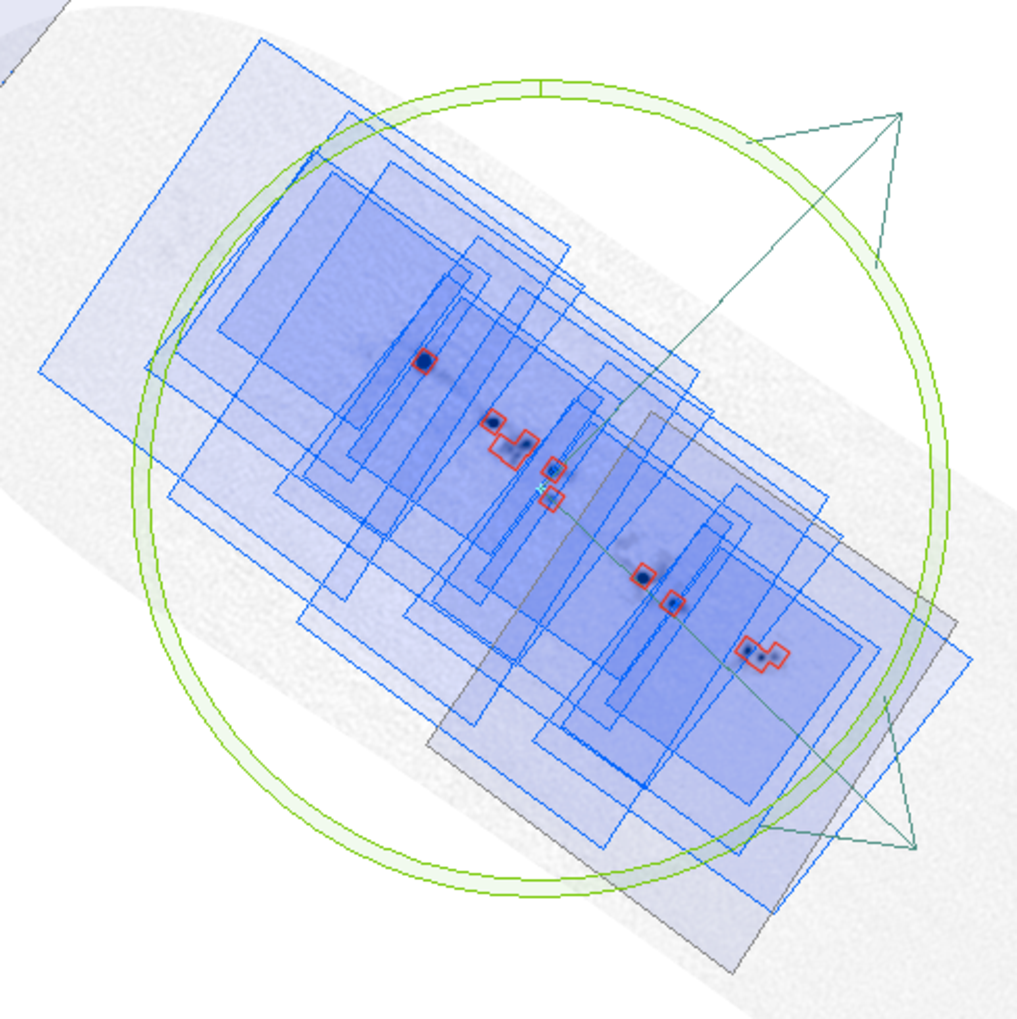
\includegraphics[width=0.6\textwidth]{thesis/images/chapters/discussion/MIRI+NIRSpec.pdf}
    \caption[Planned JWST MIRI and NIRSpec setup]{Planned JWST observations on \ngc253. The outlines of the fields to be observed with the MIRI MRS imager (blue) and NIRSpec IFU (red) are overlaid on top of the ALMA 350\,GHz dust continuum map. The central molecular gas disk is completely covered in four MIRI filters (channel $1-4$, $\sim 5-30$\,\mum) to study e.g. the dust distribution through PAH emission. The much more narrow IFU observations in the NIR are centered on the SSCs to obtain stellar properties that cannot be inferred otherwise due to extreme extinction.
    }
    \label{discussion: figure: JWST planing}
\end{figure}

The sub-mm observations of the molecular ISM described in Section~\ref{discussion: section: starburst environments} already provide a parsec scale view but ideally even higher resolution is required to resolve the clusters with a few resolution elements. For radio frequencies, either the next generation of interferometers with longer baselines and higher sensitivity (e.g. ngVLA, SKA) or very long baseline interferometry (VLBI) across continents will be able to achieve this.


%%%%%%%%%%%%%%%%%%%%%%%%%%%%%%%%%%%%%%%%%%%%%%%%%%%%%%%%%%%%%%%%%%%%%%%%%%%%%%%%%%%%%%%%%%%%%%%%%%%%

\subsection{Interaction of outflow phases}

The interaction of the different outflow phases (ionized, neutral, molecular) is poorly studied so far. 
The existence of neutral outflows traced through the \hi 21\,cm line have been discussed at low resolution in the literature for decades now \citep[e.g. M82 and NGC253][]{Boomsma:2005fa,Lucero:2015if}.
However, the relation between the two gas phases has not been addressed yet.
In some cases, such as \ngc253, the phases appear to encompass each other in the form of cone shells \citep[see Figure~\ref{introduction: figure: star formation: outflow cone},][]{2015ApJ...801...63M}. At the boundary layer between these shells energy and momentum might be exchanged and complex gas dynamics can occur.
To study this, new observations are needed. 

In \ngc253, the molecular and ionized phases are already covered by medium to high resolution observations with ALMA and integral field spectroscopic observations with VLT MUSE (P.I.: L. Zschaechner). Matching data of the neutral gas phase is, however, missing yet. 
Current facilities (VLA in its largest configuration) and planned instruments (ngVLA, SKA1 and especially SKA2) can achieve matching parsec-scale resolution in the \hi 21\,cm line.
Although technically feasible with current instruments, such an outflow phase comparison has not been tackled yet because it poses major challenges in terms of data analysis.
Since starbursts are kinematically complex environments and provide strong continuum emission, absorption against the continuum sources (young stellar clusters and AGNs if present) create a highly non-trivial spectrum composed of a mix of emission and absorption features. Disentangling the spectra and inferring robust measurements requires sophisticated analysis methods for which the outflow separation shown in Chapter~\ref{chapter: outflow} can provide the basis.
M82 povides the ideal target to obtain such a detailed view of the neutral gas for the first time.
The VLA in A configuration can achieve a resolution in 21\,cm \hi emission comparable to the molecular gas obtained with NOEMA and observations in the more compact configurations (BCD) are present already as archival data \citep{2015ApJ...814...83L,2018ApJ...856...61M}.
A similar level of detail in \hi can be achieved in \ngc253 but the southern position of \ngc253 is more challenging with the VLA.


%%%%%%%%%%%%%%%%%%%%%%%%%%%%%%%%%%%%%%%%%%%%%%%%%%%%%%%%%%%%%%%%%%%%%%%%%%%%%%%%%%%%%%%%%%%%%%%%%%%%

\section{Improved reduction and analysis techniques}
\label{discussion: section: analysis techniques}

This thesis demonstrates what can be done with state-of-the-art high-resolution data, however, this work required extensive manual work. For future instruments with higher data rates (e.g. more targets at similar quality or few targets at higher resolution) the manual work required will become the limiting factor in utilizing the data. Hence, current analysis and visualization techniques including what's shown here will have to improve. Especially when combining various datasets from a range of instruments obtained with different techniques, the challenge must not be merging the data in a consistent way to find potentially interesting details but studying said details.

The best analysis tool still is the human brain with its impressive ability to detect structure and subtle effects in datasets. Loading data into this tool is done through the eyes by visualising data. The complex 3D datasets in the sub-/millimeter/radio and more and more frequently also in optical and infrared astronomy require improved techniques to visualize higher dimensional data and allow the observer to better/easier understand the data.
This challenge was already identified within the community and is tackled from various directions. One approach is to improve the interoperability of common reduction and analysis packages. The most common platform nowadays is \texttt{python3} and large software packages are being ported to \texttt{python} \citep[e.g. SCOUSE;][]{2016MNRAS.457.2675H}, released as \texttt{python} modules \citep[e.g. \textsc{CASA};][]{McMullin:2007tj} or fitted with \texttt{python} interfaces (e.g. \textsc{IRAF}, \textsc{Gildas}) to be used seamlessly with each other and fundamental tools such as \texttt{astropy}. Although efforts have been undertaken in this direction, significant work on initial adaption and continuous maintenance remains.

With the advent of wide-band receivers in modern sub-/mm/radio telescopes, automated and reliable spectral line identification increasingly becomes a challenge. These instruments are so sensitive that dozens to hundreds of spectral lines will be routinely detected in the future. Chapter~\ref{chapter: SSCs} gives a hint on what is to come in the near future. In some regions of this datasets, the continuum is buried underneath dozens of blended lines. Continuum subtraction during data reduction and de-blending of spectral lines will need to be done automatically and robustly with minimal manual interaction. The current tools do not yet achieve this since they require careful examination of the results and regularly fail. Upgrades to even wider receivers as done for NOEMA (16\,GHz bandwidth) and discussed for ALMA ($2\times16$\,GHz) will only increase the problem.

A specific aspect of data analysis in the context of this thesis is the definition and detection of outflows that is currently very inconsistently treated among communities. The kinematic separation defined and applied in Chapter~\ref{chapter: outflow} is a first step towards fixing this issue. Other approaches in this direction are the use of machine learning techniques (e.g. Zschaechner et al., 2020, in prep.) for individual objects and statistical analyses for larger samples of resolved galaxies (e.g. in the PHANGS survey; Stuber, 2019, BSc thesis, Heidelberg University; Stuber et al., in prep.).



%%%%%%%%%%%%%%%%%%%%%%%%%%%%%%%%%%%%%%%%%%%%%%%%%%%%%%%%%%%%%%%%%%%%%%%%%%%%%%%%%%%%%%%%%%%%%%%%%%%%